\chapter{Methodology}
The task of detecting traffic rules violation can be decomposed into three abstract subtasks. They are i) Android app development, for an interface to collect the traffic rules violation videos, ii) helmet detection in the images containing motorcycles and iii) number plate detection and character recognition, for correctly fetching the license plate information of the motorcycle. The high-level architecture of the system is shown in figure \ref{fig0}.
\begin{figure}[!htb]
\centerline{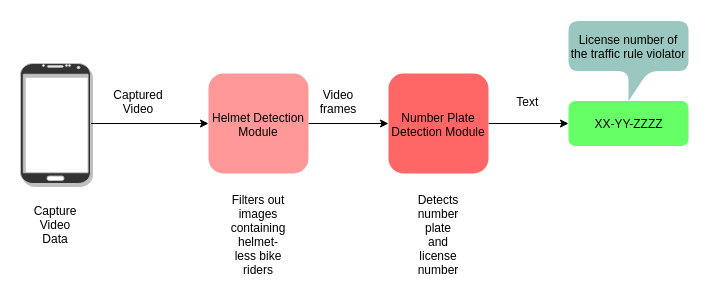
\includegraphics[height=60mm,width=132mm]{img/rd0.png}}
\caption{High-level Architecture of the Whole System}
\label{fig0}
\end{figure}

\section{Android Application}

The application is primarily used for recording video of a past incident. For this, we have used camera2 API \cite{b11} to directly access the camera device and record video. For recording past incidents we need to continuously record video and whenever a request for saving the video will come from the user, the app has to save the last 20-25 seconds of video.This is because most of the traffic rules violation incidents happen within seconds.
\begin{figure}[!htb]
\centerline{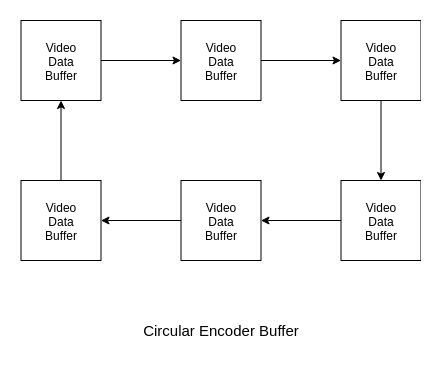
\includegraphics[height=60mm,width=92mm]{img/rd1.png}}
\caption{Architecture of Circular Encoder Buffer}
\label{fig1}
\end{figure}

\par We have created a circular buffer using a linked list which will have a size of the window as shown in figure \ref{fig1}. Here, “window” means the amount of time we want to record in the past. There will be another circular buffer which will store the metadata of the recorded video chunks. If the window size is 25 seconds then at 26th second the video data will be overwritten on the video data present at 0th second in the buffer.

\par Generally, traffic rules violation can be seen on roads while driving car or motorbike. Thus we made the whole screen as a button so that user can easily just touch the screen without much of distraction. That is while the app is open, if the user touches any part of the screen then the app will save the video up to that time of touch. The screenshots of the app’s user interface and working are given in figure \ref{fig2}.

\begin{figure}[!htb]
\centerline{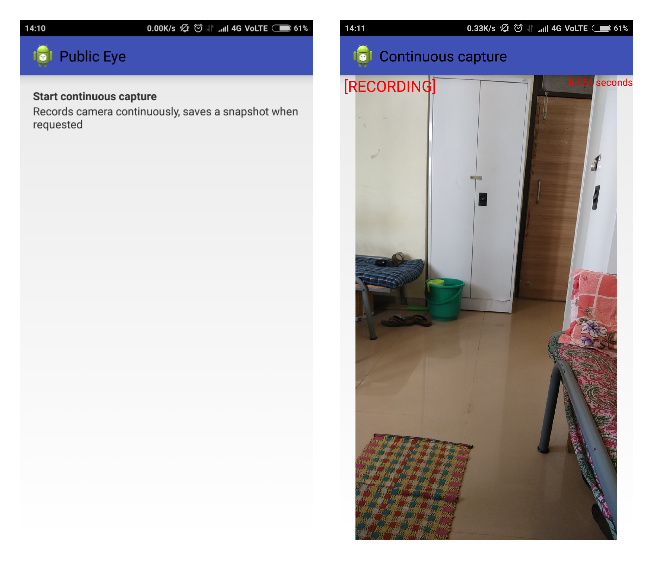
\includegraphics[height=60mm,width=92mm]{img/rd2.png}}
\caption{Screenshots of the Application}
\label{fig2}
\end{figure}


\section{Helmet Detection}
After capturing the image from our application it's now time to perform the helmet detection step. In this step, we segment the driving vehicle from the images of the dataset we feed the images to the darknet\cite{b9}. After getting the segmented images from the darknet\cite{b9} we extracted the features out of these features using different CNN architectures. After extracting the features we applied different models to classify whether a person is wearing helmet or not. We apply four different classification + Feature extracting models in doing that. Before discussing the model let's discuss the dataset we used for building these models.
\subsection{Description about the data set}
We used a dataset of total 1302 images of both helmets as well as none-helmet. We got our dataset from FullStop: Tracking unsafe stopping behavior of buses\cite{b12}. For training, we used 1074 images and 226 images for validation. We resize all the images to (224,224) pixel before feeding to the model. Our dataset is an unbiased dataset with 550 images helmet images and 524 images of non-helmet images. Our Dataset is open-source and its available at  \href{https://github.com/abhishekmaroon5/dataset2}{https://github.com/abhishekmaroon5/dataset2}. Sample images of our dataset are given in \ref{figure4}.
\begin{figure}[!htb]
\centerline{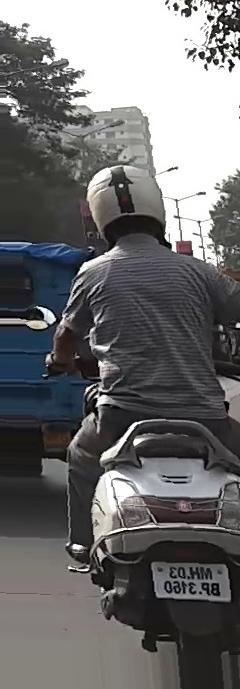
\includegraphics[height=30mm,width=22mm]{img/0_0_5402.jpg}{\\}{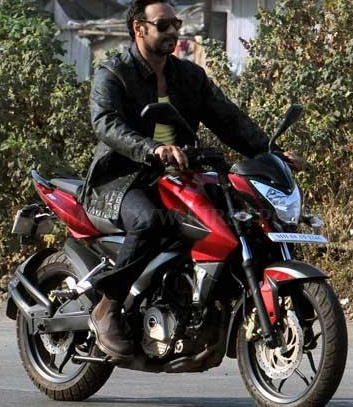
\includegraphics[height=30mm,width=22mm]{img/5577.jpg}}}

\caption{Sample images of our dataset}
\label{figure4}
\end{figure}
     
	

\subsection{Convolutional neural network from scratch(Model 1)}
In this case, we used a convolutional network of three convolution layers with ReLU activation followed by max-pooling layers in order to extract the features and in order to avoid overfitting we used to drop out of 0.5.\\ 
Code Snippet:
\begin{figure}[!htb]
\centerline{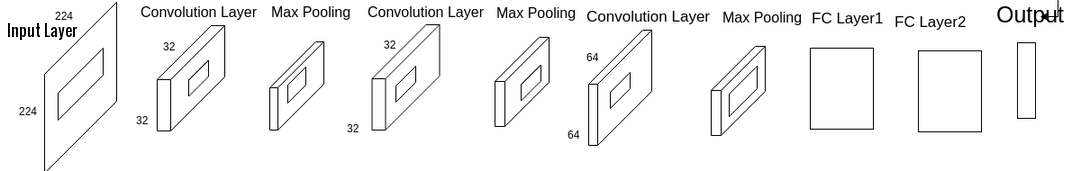
\includegraphics[height=75mm,width=162mm]{img/cnn5.png}}
\caption{Architecture of Model 1.}
\label{figcnn}
\end{figure}

\begin{lstlisting}[caption=CNN]

    model = Sequential()
    model.add(Conv2D(32, (3, 3), input_shape=(3, 150, 150)))
    model.add(Activation(`relu'))
    model.add(MaxPooling2D(pool_size=(2, 2)))
    
    model.add(Conv2D(32, (3, 3)))
    model.add(Activation(`relu'))
    model.add(MaxPooling2D(pool_size=(2, 2)))
    
    model.add(Conv2D(64, (3, 3)))
    model.add(Activation(`relu'))
    model.add(MaxPooling2D(pool_size=(2, 2)))
    \end{lstlisting}
    

{\Large Fig:  \ref{figcnn} Shows the architecture of model 1}

\subsection{Pre-trained VGG to detect bottleneck features and  Multilayer Perceptron for classification(Model 2)}
After using the model from scratch, transfer learning\cite{b7} was the other method we tried. We used the VGG16 architecture, pre-trained on the ImageNet dataset. We used only instantiate the convolutional part of the model, everything up to the fully-connected layers. We then run this model on our training and validation data once, recording the output (the `bottleneck features' from the VGG16 model: the last activation maps before the fully-connected layers). After learning the bottleneck features from above architecture we feed this to Multilayer Perceptron(MLP) of two layers in order to perform the classification task.\\
Code Snippet:
\begin{lstlisting}[caption=Pre-trained VGG]
model = applications.VGG16(include_top=False, weights=`imagenet')
generator = datagen.flow_from_directory(
train_data_dir,
target_size=(img_width, img_height),
batch_size=batch_size,
class_mode=None,
shuffle=False)
bottleneck_features_train = model.predict_generator(
generator, nb_train_samples // batch_size)
np.save(open(`bottleneck_features_train.npy', `w'),
   bottleneck_features_train)

generator = datagen.flow_from_directory(
validation_data_dir,
target_size=(img_width, img_height),
batch_size=batch_size,
class_mode=None,
shuffle=False)
bottleneck_features_validation = model.predict_generator(
generator, nb_validation_samples // batch_size)
np.save(open(`bottleneck_features_validation.npy', `w'),
bottleneck_features_validation)
\end{lstlisting}

\subsection{Pre-trained VGG to extract bottleneck features and Support Vector Machine for classification (Model 3)}
Extracting the bottleneck features from the previous step is same in this step also. After extracting the features we performed Support vector machine classification using all the features we got from the previous step and trained it on multiple learning rates using Stochastic Gradient Descent.
We use the same code as above to extract the features. We also tried different kernelized  SVM's such Linear, RBF(Radial basis function), etc.
\subsection{Fine-tuning the top layers of a pre-trained network (Model 4)}

\par We firstly instantiate the convolutional base of VGG16 and load its weights. After that, we freeze the layers of the VGG16 model up to the last convolutional block and after that, we add our previously defined fully-connected model on top and load its weights. We choose to only fine-tune the last convolutional block rather than the entire network in order to prevent overfitting since the entire network would have a very large entropic capacity and thus a strong tendency to overfit. The features learned by low-level convolutional blocks are more general, less abstract than those found higher-up, so it is sensible to keep the first few blocks fixed (more general features) and only fine-tune the last one (more specialized features).
\\Code Snippet:
\begin{lstlisting}[caption = Put some caption]
   model=applications.VGG16(include_top=True,weights=`imagenet',input_shape = (img_width,img_height,3)
   print(``Model Loaded!!!'')
                   last_layer = model.get_layer(`block5_pool').output
                                   x= Flatten(name=`flatten')(last_layer)
                   x = Dense(256, activation=`relu', name=`fc1')(x)
   x = Dense(1, activation=`sigmoid', name=`fc2')(x)
   out = Dense(num_classes, activation=`softmax', name=`output')(x)
   custom_vgg_model = Model(model.input, out)
   print(custom_vgg_model.summary())

   for layer in custom_vgg_model.layers[:-3]:
            layer.trainable = False

   custom_vgg_model.layers[3].trainable

   custom_vgg_model.compile(loss=`sparse_categorical_crossentropy',optimizer=`rmsprop',metrics=[`accuracy'])

   test_generator = datagen.flow_from_directory(
       validation_data_dir,
       target_size=(img_width, img_height),
       batch_size=batch_size,
       class_mode=`binary' ,shuffle=True)

\end{lstlisting}




\section{Number Plate Detection}
After detecting the helmetless bike riders we want to detect their license number for reporting. Here, we have proposed two methods to perform this task. They are described below.
\subsection{Method 1}
In this method, we have implemented the number plate detection module which has three components such as : 
\begin{itemize}
    \item Number plate localization.
    \item Character segmentation.
    \item Character recognition.
\end{itemize}
\par The architecture of the method is given in figure \ref{fig12}.
\begin{figure}[!htb]
\centerline{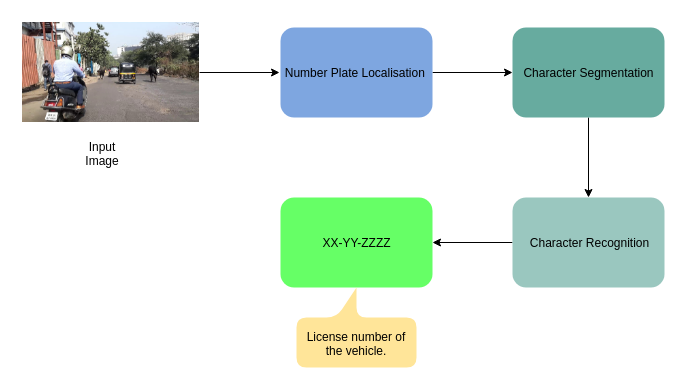
\includegraphics[height=40mm,width=82mm]{img/rd12.png}}
\caption{Architecture of Number Plate Detection Module in Method 1}
\label{fig12}
\end{figure}
\subsubsection{Number plate localization}
In this step we figure out the position of the number plate in the image. The input in this step is an image of vehicle and output is the license plate. 
\par First, we have converted the input image into gray-scale image where the value of each pixel in the image is between 0 to 255. After that we need to binarize the image where each pixel is either black or white. We are binarizing the image to find connected components in the image. The code to binarize the image is given below : 
\begin{lstlisting}[caption=Image binarization]
car_image = imread(`car.jpg', as_grey=True)
gray_car_image = car_image * 255
threshold_value = threshold_otsu(gray_car_image)
binary_car_image = gray_car_image > threshold_value
\end{lstlisting}
\begin{figure}[!htb]
\centerline{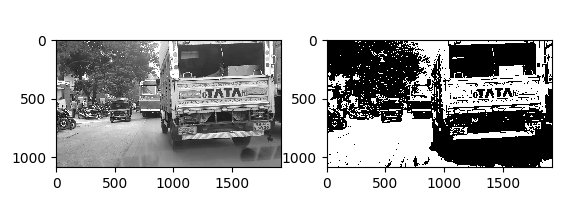
\includegraphics[height=60mm,width=132mm]{img/rd3.png}}
\caption{Grayscale and Binary Image}
\label{fig3}
\end{figure}


 \par After this, we need to perform connected component analysis (CCA) to find out the connected regions in the binary image. CCA helps us to locate and label the connected regions in the foreground of the binary image. 
 \begin{itemize}
     \item \textbf{Connected component analysis (CCA)} is an algorithm to find the connected components in an image. Here the concept of connected components from graph theory has been used. Connected components of a graph is defined as the sub-graph where each vertex in it are connected with each other via some path but not connected to the vertices of other sub-graphs. In CCA, each connected component is uniquely labeled and can be classified as some objects in the foreground of the binary image. 
 \par The algorithm of CCA is described below. 
 \begin{lstlisting}
 Iterate over all the pixel in the binary image row-wise.
 If the element is not in the background then : 
    Get the neighbor pixels of the current pixel.
    If there are no neighbors then : 
        Uniquely label the current pixel.
    Else :
        Find a neighbor with the smallest label.
        Assign that label to the current pixel.
    Store the equivalence between neighboring pixels in some table.
    Iterate through all the pixels in a row-wise manner.
    If the pixel is not in background then : 
        Relabel the pixel with lowest equivalent label.
 \end{lstlisting}
 The neighborhood of a pixel is determined by 8-connectivity of that pixel, i.e, its potential neighbors (black dots) are shown in figure \ref{fig4}. 
\begin{figure}[!htb]
\centerline{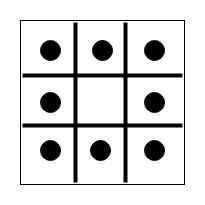
\includegraphics[height=40mm,width=40mm]{img/rd4.png}}
\caption{8-connectivity neighbors}
\label{fig4}
\end{figure}
 
 \par One example of CCA is given in figure \ref{fig5}.
 
 \begin{figure}[!htb]
\centerline{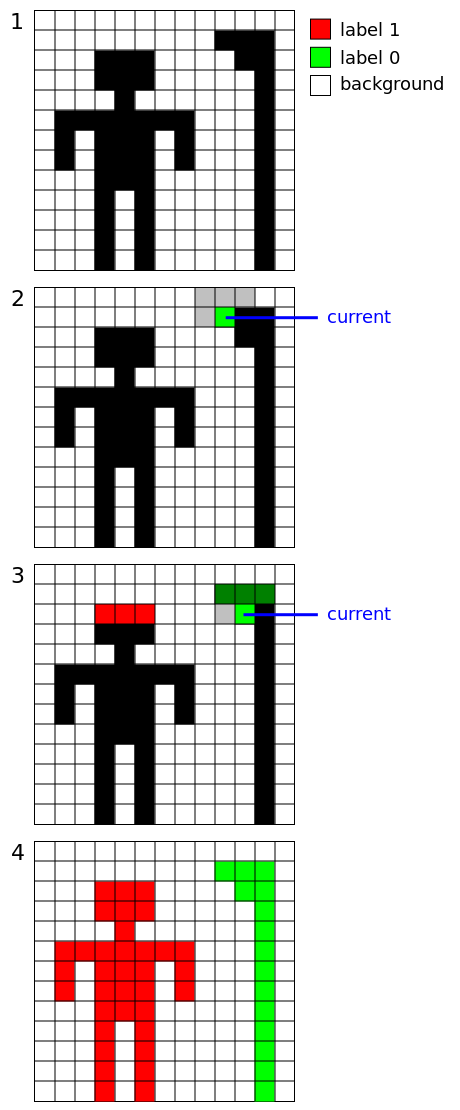
\includegraphics[height=80mm,width=45mm]{img/rd5.png}}
\caption{Example of CCA \cite{b1}}
\label{fig5}
\end{figure}
 
 \par In our project we have used $skimage$ \cite{b14} module to do CCA on the binary image. The code snippet of this part is given below : 
 \begin{lstlisting}[caption=Connected component analysis]
label_image = measure.label(localization.binary_car_image)
for region in regionprops(label_image):
    if region.area < 50:
        continue
    minRow, minCol, maxRow, maxCol = region.bbox
    rectBorder = patches.Rectangle((minCol, minRow), maxCol-minCol, maxRow-minRow, edgecolor=`red', linewidth=2, fill=False)
 \end{lstlisting}
 In the above code snippet, $measure.label$ is mapping all the connected regions and labeling them and $regionprops()$ method returns the list of all the regions and as well as their properties like area, label, bounding box, etc. The resulting images after this step is given in figure \ref{fig6}.
\begin{figure}[!htb]
\centerline{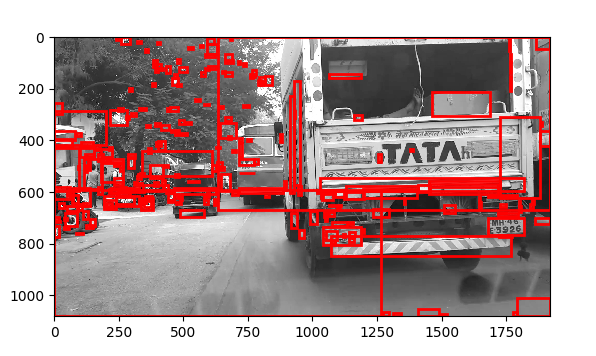
\includegraphics[height=60mm,width=90mm]{img/rd6.png}}
\caption{Detection of Connected Regions using CCA on a Sample IMage}
\label{fig6}
\end{figure} 
 
 
 
Now, there are many regions which do not contain the number plate but got selected in the previous step. So, we need to filter out the number plate like regions out of all the region proposals. We have identified some features of the Indian number plates such that : 
 \begin{itemize}
     \item The number plates are rectangular but they are more like a square, i.e, the height and width of the number plates does not have much difference.
     \item The proportion of the height of the number plate region to the full image ranges from 3\% to 10\%.
     \item The proportion of the width of the number plate region to the full image ranges from 4\% to 11\%.
 \end{itemize}
 \par We applied the above observed characteristics to filter out the potential number plate regions out of the image. The code snippet for filtering is given as : 
 \begin{lstlisting}[caption=Number Plate Filtering]
 plate_dimensions = (0.03*label_image.shape[0], 0.1*label_image.shape[0], 0.04*label_image.shape[1], 0.11*label_image.shape[1])
min_height, max_height, min_width, max_width = plate_dimensions
plate_objects_cordinates = []
plate_like_objects = []
for region in regionprops(label_image):
    if region.area < 50:
        continue
    min_row, min_col, max_row, max_col = region.bbox
    region_height = max_row - min_row
    region_width = max_col - min_col
    if region_height >= min_height and region_height <= max_height and region_width >= min_width and region_width <= max_width and region_width > region_height:
        plate_like_objects.append(localization.binary_car_image[min_row:max_row,
                                  min_col:max_col])
        plate_objects_cordinates.append((min_row, min_col,
                                              max_row, max_col))
        rectBorder = patches.Rectangle((min_col, min_row), max_col-min_col, max_row-min_row, edgecolor=``red", linewidth=2, fill=False)
 \end{lstlisting}
 \end{itemize}
 
 \vspace{.3in}
 The result of filtering is shown in figure \ref{fig8}.
 
% \begin{figure}[!htb]
% \centerline{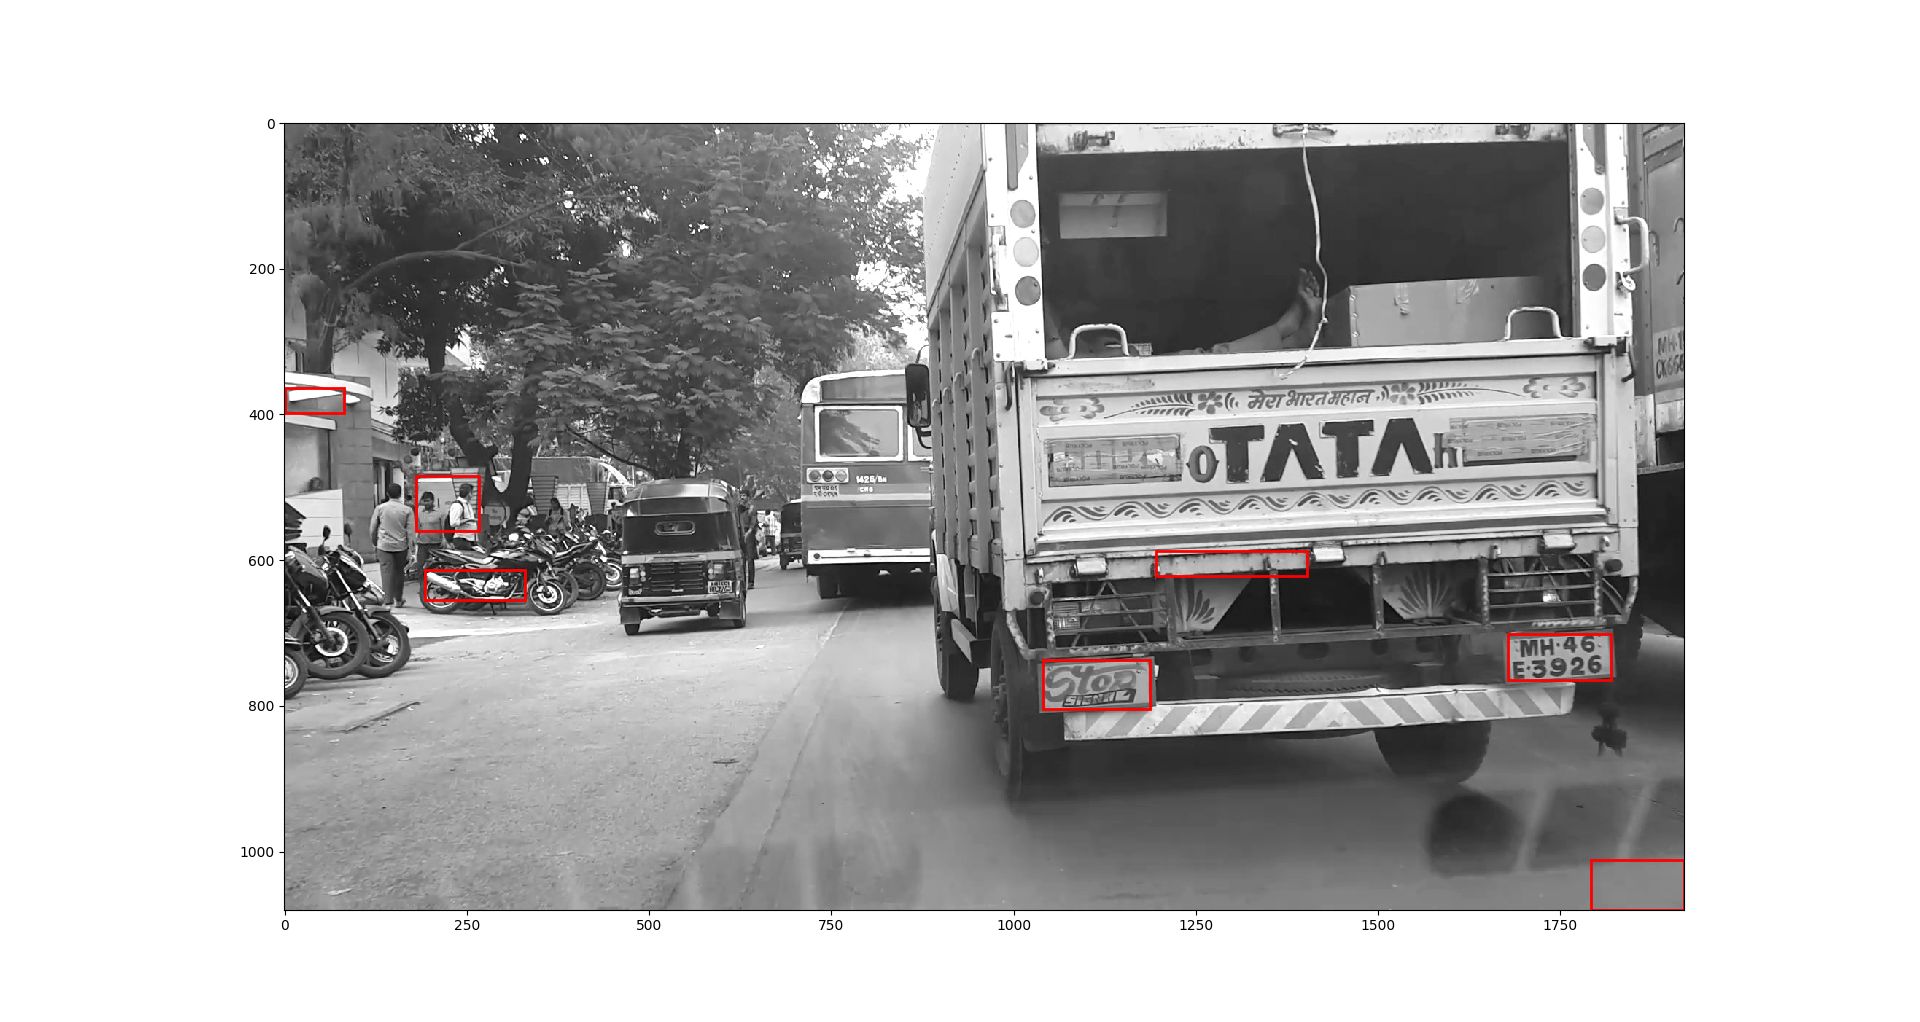
\includegraphics[height=70mm,width=140mm]{img/rd7.png}}
% \label{fig7}
% \end{figure}

\begin{figure}[!htb]
\centerline{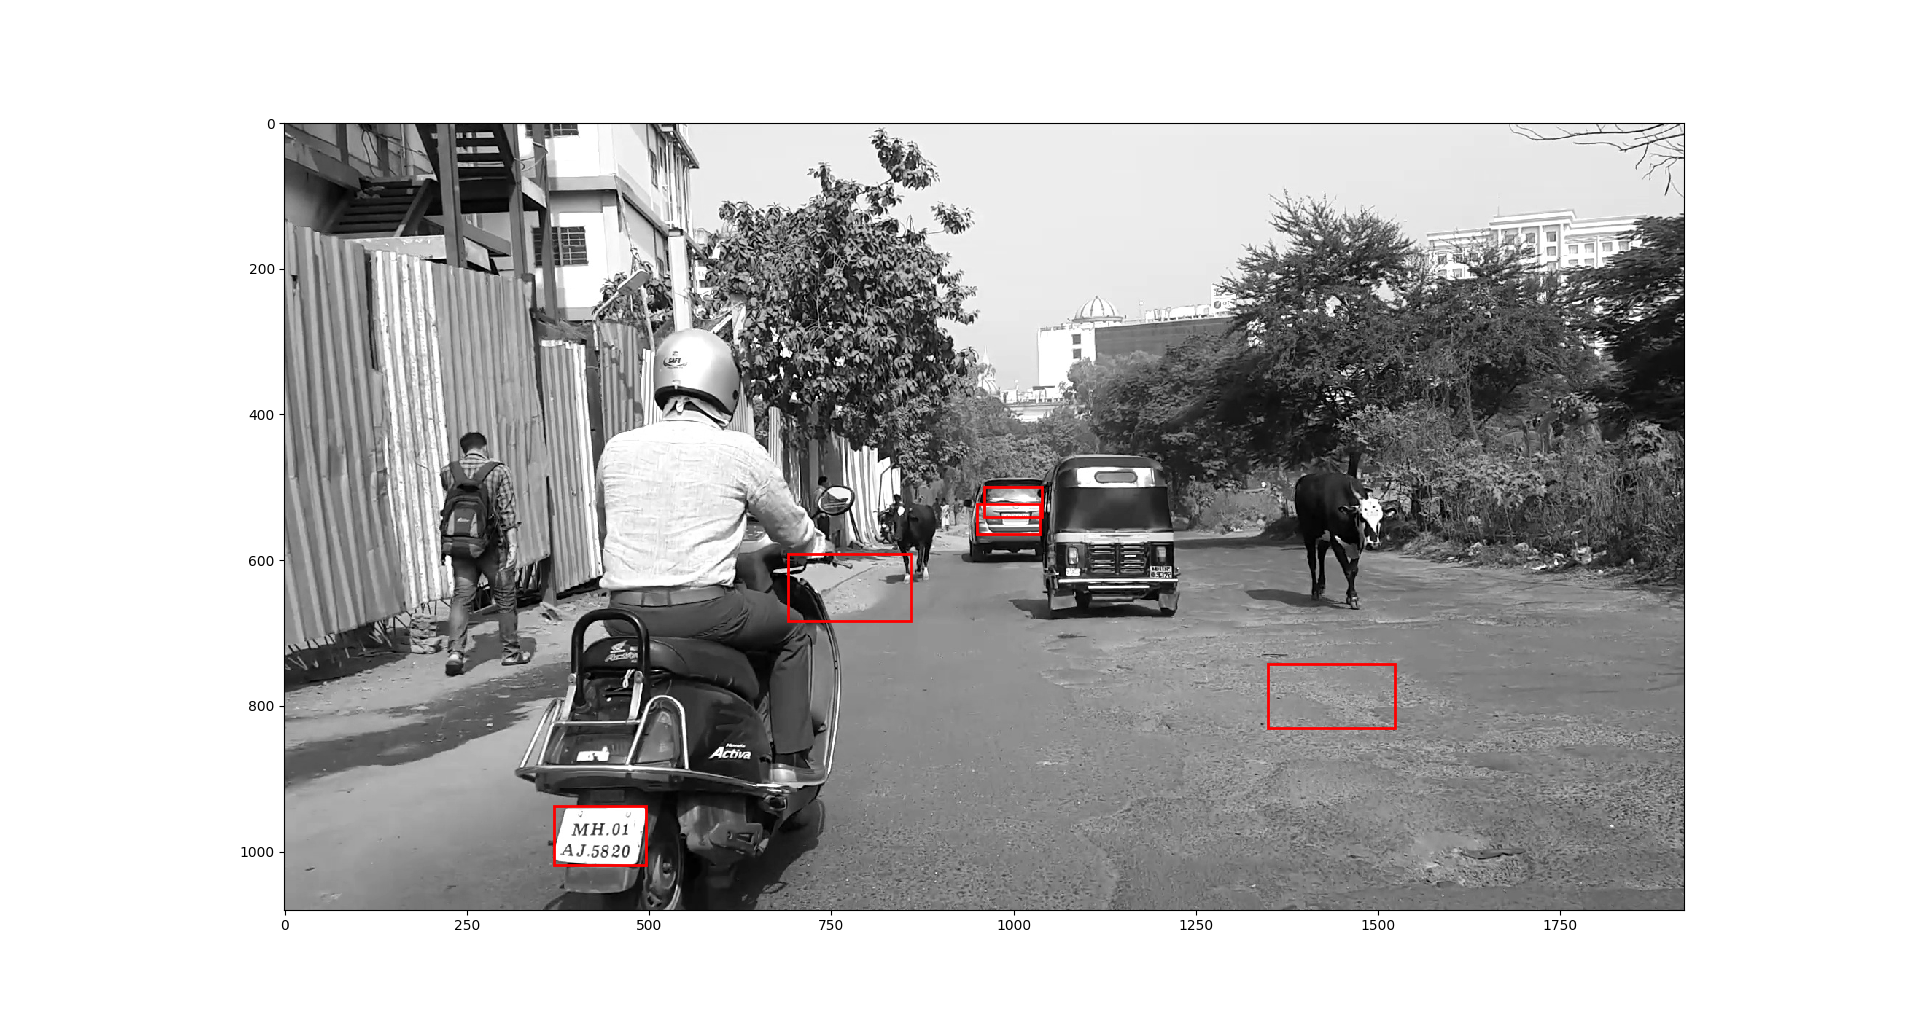
\includegraphics[height=70mm,width=140mm]{img/rd8.png}}
\caption{Relevant Regions Filtered Out By CCA}
\label{fig8}
\end{figure}
 
 
\subsubsection{Character Segmentation}

Number plate localization will produce several number plate region proposals. Now, to do character segmentation on the number plate image we have to first filter out the actual number plate out of all the proposals. To filter out the actual number plate we do a summation of all the pixels along the column. This summation will show that number plate patch will stand out as it has lots of objects in it. Thus the values after summation of pixel intensities will also be high. 
\par After getting the binary image of the number plate we perform CCA again. The CCA algorithm will detect the objects present in the binary image of the number plates. Here the "objects" are the characters present in the number plate. A sample result of this stage is shown in the figure \ref{fig9}.

\begin{figure}[!htb]
\centerline{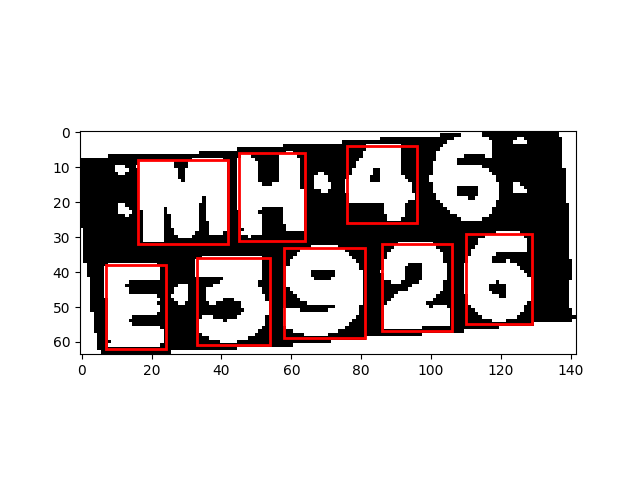
\includegraphics[height=70mm,width=140mm]{img/rd9.png}}
\caption{Character Segmentation Example}
\label{fig9}
\end{figure}
 
 
\subsubsection{Character Recognition}
After segmenting the characters out of the number plate we have to just recognize them. This recognition step has been done with the help of machine learning. We have trained a support vector machine with 360 training samples. Our training data consists of 10 images of size $20*20$ pixels for each alphabet and digit. After completion of training the trained model was saved as a .pkl file and deployed for test data. This trained model will produce text output when test data will be feeded. 
\par The segmented character images will be reshaped to size $20*20$ pixels because all the training data images are also of size $20*20$ pixels. A sample result is shown in the figure \ref{fig10}.

\begin{figure}[!htb]
\centerline{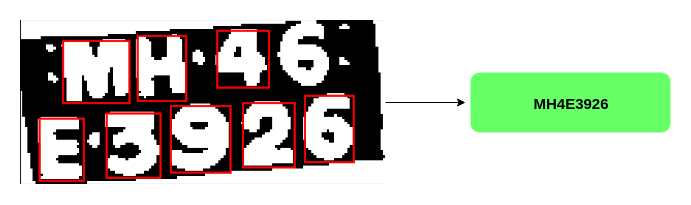
\includegraphics[height=40mm,width=140mm]{img/rd10.png}}
\caption{Segmented Characters to Text Example}
\label{fig10}
\end{figure}

\par The `6' that is missing is connected to the upper white region of the segmented image. That is why it became a whole connected component and crossed the threshold of height and width of a character.
 

\subsection{Method 2}

There are many open source softwares which can be used as a black box to detect number plates. We have used one such software called OpenALPR \cite{b0}. We have used their API calls to upload a picture and get results, i.e, the number plate location will be detected and also the license number will be sent as output. This software is using Google Tesseract \cite{b12} for character recognition. The performance of this software is given in table 4.2.2.





